%%%%%
%%
wa%% Sample document ``thesis.tex''
%%
%% Version: v0.2
%% Authors: Jean Martina, Rok Strnisa, Matej Urbas
%% Date: 30/07/2008
%%
%% Copyright (c) 2008-2011, Rok Strniša, Jean Martina, Matej Urbas
%% License: Simplified BSD License
%% License file: ./License
%% Original License URL: http://www.freebsd.org/copyright/freebsd-license.html
%%%%%

% Available documentclass options:
%
%   <all `report` document class options, e.g.: `a5paper`>
%   withindex   - enables the index. New index entries can be added through `\index{my entry}`
%   glossary    - enables the glossary.
%   techreport  - typesets the thesis in the technical report format.
%   firstyr     - formats the document as a first-year report.
%   times       - uses the `Times` font.
%   backrefs    - add back references in the Bibliography section
%
% For more info see `README.md`
\documentclass[times, withindex, backrefs, firstyr]{cam-thesis}
\usepackage[dvipsnames]{xcolor} 

% Citations using numbers
\usepackage[numbers]{natbib}
\usepackage[disable]{todonotes}
% \usepackage[colorinlistoftodos,textsize=tiny,textwidth=0.7in]{todonotes}

\usepackage{booktabs}
\usepackage{graphicx}
\usepackage{caption}
\usepackage{subcaption}
\usepackage{url}            % simple URL typesetting
\usepackage{booktabs}       % professional-quality tables
\usepackage{amsmath}       % blackboard math symbols
\usepackage{amsfonts}       % blackboard math symbols
\usepackage{nicefrac}    
\usepackage{setspace}
\usepackage{algorithm}

\usepackage[noend]{algpseudocode}

\algrenewcommand\algorithmicindent{2em}

\algnewcommand\algorithmicforeach{\textbf{for each}}
\algdef{S}[FOR]{ForEach}[1]{\algorithmicforeach\ #1\ \algorithmicdo}

 
\usepackage[normalem]{ulem}
\useunder{\uline}{\ul}{}

%%%%%%%%%%%%%%%%%%%%%%%%%%%%%%%%%%%%%%%%%%%%%%%%%%%%%%%%%%%%%%%%%%%%%%%%%%%%%%%%
%% Thesis meta-information
%%

%% The title of the thesis:
% \setuptodonotes{inline,noinlinepar,inlinewidth=0.15\textwidth}
\usepackage[capitalise]{cleveref}
\usepackage{pdfpages}

\title{Bidirectional Hierarchical Federated Learning}

%% The full name of the author (e.g.: James Smith):
\author{Alexandru-Andrei Iacob}

%% College affiliation:
\college{Homerton}

%% College shield [optional]:
% \collegeshield{CollegeShields/Christs}
% \collegeshield{CollegeShields/Churchill}
% \collegeshield{CollegeShields/Clare}
% \collegeshield{CollegeShields/ClareHall}
% \collegeshield{CollegeShields/CorpusChristi}
% \collegeshield{CollegeShields/Darwin}
% \collegeshield{CollegeShields/Downing}
% \collegeshield{CollegeShields/Emmanuel}
% \collegeshield{CollegeShields/Fitzwilliam}
% \collegeshield{CollegeShields/Girton}
% \collegeshield{CollegeShields/GonCaius}
\collegeshield{CollegeShields/Homerton}
% \collegeshield{CollegeShields/HughesHall}
% \collegeshield{CollegeShields/Jesus}
% \collegeshield{CollegeShields/Kings}
% \collegeshield{CollegeShields/LucyCavendish}
% \collegeshield{CollegeShields/Magdalene}
% \collegeshield{CollegeShields/MurrayEdwards}
% \collegeshield{CollegeShields/Newnham}
% \collegeshield{CollegeShields/Pembroke}
% \collegeshield{CollegeShields/Peterhouse}
% \collegeshield{CollegeShields/Queens}
% \collegeshield{CollegeShields/Robinson}
% \collegeshield{CollegeShields/Selwyn}
% \collegeshield{CollegeShields/SidneySussex}
% \collegeshield{CollegeShields/StCatharines}
% \collegeshield{CollegeShields/StEdmunds}
% \collegeshield{CollegeShields/StJohns}
% \collegeshield{CollegeShields/Trinity}
% \collegeshield{CollegeShields/TrinityHall}
% \collegeshield{CollegeShields/Wolfson}
% \collegeshield{CollegeShields/CUniNoText}
% \collegeshield{CollegeShields/FitzwilliamRed}

%% Submission date [optional]:
% \submissiondate{November, 2042}

%% You can redefine the submission notice [optional]:
% \submissionnotice{A badass thesis submitted on time for the Degree of PhD}

%% Declaration date:
\date{29 June, 2023}

%% PDF meta-info:
\subjectline{Computer Science}
\keywords{one two three}



%%%%%%%%%%%%%%%%%%%%%%%%%%%%%%%%%%%%%%%%%%%%%%%%%%%%%%%%%%%%%%%%%%%%%%%%%%%%%%%%
%% Glossary [optional]:
%%
% \newglossaryentry{HOL}{
    name=HOL,
    description={Higher-order logic dasdasdas }
}




%%%%%%%%%%%%%%%%%%%%%%%%%%%%%%%%%%%%%%%%%%%%%%%%%%%%%%%%%%%%%%%%%%%%%%%%%%%%%%%%
%% Contents:
%%
\begin{document}



%%%%%%%%%%%%%%%%%%%%%%%%%%%%%%%%%%%%%%%%%%%%%%%%%%%%%%%%%%%%%%%%%%%%%%%%%%%%%%%%
%% Title page, abstract, declaration etc.:
%% -    the title page (is automatically omitted in the technical report mode).
\frontmatter{}
%%%%%%%%%%%%%%%%%%%%%%%%%%%%%%%%%%%%%%%%%%%%%%%%%%%%%%%%%%%%%%%%%%%%%%%%%%%%%%%%
%% Thesis body:
%%
\chapter{Introduction}

Federated Learning (FL) is a distributed Machine Learning (ML) paradigm allowing multiple clients to train a shared collaborative model without communicating private data. It was introduced by \citet{FedAvg} as a means of reducing communication costs and lessening the privacy concerns of storing sensitive data in a centralised location, following the principle of data minimisation outlined in the \citet{White_House_Report} privacy report. These properties have led to FL applications with large cohorts of small edge devices, e.g., mobile keyboard prediction~\citep{GoogleKeyboard} for Android phones, and settings with larger entities subject to privacy requirements, e.g., hospitals~\citep{FLmedicine}. \citet{AdvancedAndOpenProblems} distinguish them as cross-device and cross-silo FL\@.

The growth in the preponderance of Federated Learning since the publication of \citet{FedAvg} can be ascribed to two primary trends. First, an increase in the privacy requirements of consumers and legal frameworks has put pressure on technology companies. This pressure drove interest in privacy-preserving ML at major corporations such as Google~\citep{FedAvg,GoogleKeyboard,tensorflowfederated,PracticalPrivateFLkairouz21b}, Microsoft~\citep{FLINT,Flute}, Meta~\citep{PAPAYA,FedBuff}, and Apple~\citep{AppleFL}. Second, ML has extended to domains with strict privacy requirements such as healthcare~\citep{FLmedicine,FutureOfHealth,BigDataCancer}, Human Activity Recognition~(HAR)~\citep{HARusingFL_2018,ClusterFL} or collaborations between competing corporations~\citep{SustainableIncentive,TowardsFairPrivacyPreservingFL}. Moreover, the emergence of Large Language Models (LLMs)~\citep{OpportunitiesAndRisksLLM} has made accessing private language corpora advantageous, leading to the development of Federated Natural Language Processing (FedNLP)~\citep{FedNLP}. Similarly, the release of openly available LLM pre-trained weights~\citep{LLaMA} allows collaboration between entities with low computational resources using FL frameworks~\citep{Flower,FedScale,FedML}.

While the field has enjoyed abundant scientific and industry attention, the privacy and communication benefit it provides cause significant challenges in efficiently scaling and evolving federated systems. Crucially, training a single global model is unsuitable when unusual clients require partial or complete personalisation of the model to their local data distribution.

In its standard form, FL operates directly on clients using a centralised server to distribute model parameters and then aggregate them after client training; this process is repeated for multiple rounds. However, data in FL is subject to attributes such as client geographic location, sensor hardware, and behaviour. Due to these factors, the federated distribution violates the Independent and Identically Distributed (IID) assumption. Such \emph{data heterogeneity}~\citep[sec. 3.1]{AdvancedAndOpenProblems} is interwoven with \emph{systems heterogeneity}~\citep[sec. 7.2]{AdvancedAndOpenProblems} since clients have different computational abilities and network speeds. Additionally, the communication costs of transmitting model parameters between servers and clients are non-trivial.
% Since data heterogeneity makes obtaining a single global model efficient on all client data distributions unfeasible, we are concerned with creating arbitrary levels of personalisation in the form of Hierarchical Federated Learning in a manner that improves learning efficiency and allows such systems to evolve.

Efficiency and scalability have been at the centre of FL research since \citet{GoogleKeyboard} applied FL to mobile keyboard prediction at Google. Building on top of \citet{GoogleKeyboard}, \citet{ScaleSystemDesign} showed that FL could be used to train models over tens of millions of smartphones. However, despite the optimistic billion-device forecasts of \citet{ScaleSystemDesign}, several limitations to the efficiency of FL emerged. These limitations are threefold: (a) synchronous FL can only effectively use hundreds of devices every round, (b) federated training is considerably slower than centralised training, (c) user devices are unreliable, leading to dropout and stragglers. These limitations received further attention in the empirical evaluation of \citet{LargeCohorts}.

\citet{LargeCohorts} show that the performance of FL does not scale as expected when the number of clients trained every round increases despite previous theoretical work~\citep{TighterTheory} indicating the contrary. Their experimental results show that the primary limitation of increasing cohort size under Non-IID settings is the miss-alignment of client models, indicated by a near-zero cosine similarity between updates. This miss-alignment limits the impact of a round, causes diminishing returns to increasing cohort size, and results in an inability to learn efficiently from client data in parallel. Thus, given that FL is highly parallel, its scalability is limited by the ability to learn from clients on a per-sample basis. Asynchronous Federated Learning systems~\citep{AsynchronousFLonHetDevicesSurvey,FedBuff,AsyncrhonousOnlineFL,AsyncDropout}, such as Meta's PAPAYA~\citep{PAPAYA}, show promise in improving efficiency and scalability; however, they introduce the new issues of staleness and high update variance.

Evolving FL systems is also a major challenge. The datasets of clients forming a federated network are generally not static. Clients may delete data immediately after generation, periodically, or ad-hoc based on memory needs or owner requests. Furthermore, the characteristics of newly added data can change gradually or immediately. For example, seasonal transitions shift captured images slowly, while changing locations leads to discrete changes. This problem is known as dataset shift~\citep[sec. 3.1]{AdvancedAndOpenProblems} and represents \emph{intra-client} heterogeneity rather than the common \emph{inter-client} heterogeneity. Even works which maintain persistent local models~\citep{Ditto,FlWithPersonalisationLayers,AdaptivePersonalisedFederatedLearning,FederatedLearningMixtureOfGlobalAndLocal} assume that this model is only used within FL rounds, obfuscating such shifts.\\

\noindent \textbf{Structure:} Given the challenges of FL and shortcomings of previous work, detailed in \cref{sec:back} with my completed work in \cref{sec:completed_work}, the proposed research for my PhD aims to \emph{provide flexible personalisation for highly efficient and scalable FL systems} by exploring the research questions outlined in \cref{sec:proposal:research_questions}. To achieve this goal, \cref{sec:proposal} propose a new family of FL algorithms called Bidirectional Hierarchical Federated Learning (B-HFL) based on \cref{alg:B-HFL}. Building on these foundations, I outline the research directions of my PhD that B-HFL enables in \cref{sec:proposal:research_directions}. Finally, I provide a detailed timeline for the PhD in \cref{sec:timeplan}.

\noindent \textbf{Notice:} The following subsection provides a \emph{summary} of B-HFL and the contributions it enables.
\section{Summary of Proposed Research}
Bidirectional Hierarchical FL (B-HFL) will address the aforementioned personalisation, efficiency, and evolution challenges by constructing hierarchical federated network structures that allow bidirectional and potentially cyclical dataflow where each leaf is a client and each internal node is a server. As a result, levels in the tree closer to the leaves are more personalised to the specific client population of a subtree, and those closer to the root provide more generalisable models. Furthermore, since B-HFL treats nodes homogeneously, every intermediary node can operate independently like a standard FL server, using synchronous or asynchronous execution of its sub-nodes depending on constraints.

This proposal builds upon the work done by \citet{EuroMLSysWorkshop} and \citet{OperaWorkshop} on personalised and hierarchical FL. The proposed system communicates data in as shown in \cref{alg:B-HFL} and \cref{fig:TreeStructure}. Crucially, model parameters can flow bidirectionally, and nodes can apply partial updates from their parents via aggregation. Furthermore, each node can weight children and parent parameters differently while using methods such as the adaptive server optimisers~\citep{FedOPT}, model-interpolation~\citep{AdaptivePersonalisedFederatedLearning,FederatedLearningMixtureOfGlobalAndLocal}, or training-based methods~\citep{Ditto,EWC,DeepMutualLearning,PersonalisedFLFirstOrder}. Adaptive algorithms and model interpolation are particularly relevant as they allow each node in the tree to distinguish itself based on its previous state without necessitating additional parameter tuning. Furthermore, since each edge-server controls fewer clients, the diminishing effects of increasing cohort sizes are avoided.  Finally, in the case where client cohorts are meaningfully clustered, this structure may allow a drastic increase in the sample efficiency of the system as each cluster decides how to optimise the generalisation-personalisation trade-off~\citep{PersonalisationGeneralisationTradeoff,Auxo}. The potential contributions to the field of Federated Learning include:
\begin{enumerate}
    \item A family of efficient algorithms with minute control of personalisation and generalisation, capable of achieving communication efficiency in hierarchical networks.
    \item The investigation of three techniques enabled by B-HFL\@: (a) allowing leaf nodes to maintain persistent local models training asynchronously to tackle dataset shift, (b) making any node in the tree capable of training with a proxy dataset to inject general information, (c) constructing  vertical connections in the tree, similar to residual connections~\citep{ResNet}, to allow customisable dataflow without changing the underlying communication infrastructure.
    \item Extensive empirical evaluations considering scenarios with or without meaningful client clusters in language and image/speech recognition tasks leading to intended publication at \href{https://iclr.cc/}{ICLR} or \href{https://mlsys.org/}{MLSys}. This publication will be followed up by a work intended for \href{https://sigmobile.org/mobicom/2023/}{MobiCom} investigating asynchronous training on resource-constrained devices with dataset shift using the Raspberry Pi FL cluster at Cambridge ML Systems.
\end{enumerate}










\chapter{Background and Related Work}\label{sec:back}
The standard FL objective can be modelled as seen in \cref{eq:flObjective}
\begin{equation} \label{eq:flObjective}
    \underset{\theta}{\min} F(\theta) = \sum_{c \in C} p_c F_c(\theta) \ ,
\end{equation}
where \(F\) is the federated objective, $C$ is the client set, $\theta$ is the model, and \(F_c\) is the loss of client \(c\) weighted by their fraction of the total number of examples $p_c$. This formulation assumes that a single global model is being trained without regard for the distribution of its performance across client datasets. Federated Averaging (FedAvg)~\citep{FedAvg} trains the global model locally, for each round $t$ it sums the update \(\theta_t^c - \theta_t\) from client $c$ weighted by \(p_c\) with the previous model \(\theta_t\) using learning rate \( \eta \), as seen in \cref{eq:FedAvg}
\begin{equation} \label{eq:FedAvg}
    \theta_{t+1} = \theta_t + \eta \left( \sum_{c \in C} p_c \left(\theta_t^c - \theta_t \right) \ \right) \ .
\end{equation}
The inability to colocate client data and the need to construct rough mixtures of model parameters as a compromise represent the leading causes of FL-specific challenges.

\section{Heterogeneity}\label{background:data_heterogeneity}

Non-IID data has been shown to impact both practical accuracies \citep{FLwithNonIID, NonIIDQagmire} and theoretical convergence bounds \citep{OnTheConvergenceOfFedAvgOnNonIIDdata}. It is thus worth detailing some forms of heterogeneity that \citet{AdvancedAndOpenProblems} identify. The most commonly addressed form is quantity skew caused by clients having different amounts of data available. Standard FL algorithms effectively address Quantity skew via a simple reweighing (\cref{eq:FedAvg}). The other frequently-considered type of heterogeneity is label-distribution skew which is quantity skew per class. While these forms of heterogeneity have been most investigated, situations where features and labels are not related in the same manner across clients are more pathological and may require some form of clustering or personalisation to tackle. In the worst-case scenario, each client may represent an entirely different task, as in Multi-Task Learning, with potentially little overlap in their solution space.


\paragraph{System (hardware) heterogeneity} Devices within the federated network may differ regarding computational ability, storage, network speed, and reliability. They may also differ from themselves at a different point in time as their battery power, network connection, or operational mode vary. Importantly, variations in data-generating hardware, such as sensors, are linked to data heterogeneity. However, system heterogeneity and device unreliability harm the FL process independently of data. For example, slower hardware may result in straggling clients which elongate rounds in synchronous FL~\citep{ScaleSystemDesign,FedProx} or operate on stale parameters in asynchronous FL~\citep{AsyncFedOpt,PAPAYA}\@. In addition, network or device unreliability creates client dropout, which requires oversampling clients~\cite{ScaleSystemDesign} and harms the effectiveness of maintaining local state across rounds.

\paragraph{Dataset Shift and Continual Learning}  Allowing ML models to participate in lifelong learning effectively is the goal of continual learning~\citep{ContinualLearningSurvey}; however, applying continual learning to the FL context is problematic for two primary reasons. First, the optimisation objective~(\cref{eq:flObjective}) intends to find a compromise model across all clients and cannot precisely fit all their data. Consequently, if the dataset of one client shifts independently of the whole network, the federated model will find it hard to adapt. Second, continual learning techniques such as Elastic-weight Consolidation~\citep{EWC}, PackNet~\citep{PackNetAM}, and Learning without Forgetting~\citep{LearningWithoutForgetting} are designed for task-incremental settings where class labels are known, small amounts of previous data may still be available for specialised use cases~\citep{EWC}, or there may even be different output heads for each task. The privacy requirements of FL make such solutions difficult at the level of the federated network without the addition of persistent local storage.
\section{Privacy}
While privacy in FL is not currently the intended primary research direction for the near-term of my PhD, it is one of the primary concerns of the field. As such, any approaches which attempt to tackle the main challenges of FL must do so while accounting for their privacy implications.

Since FL keeps training data locally stored on the client, it offers more privacy than standard ML approaches. However, previous works~\citep{InvertingGradients,ProtectionAgainstReconstructionAndItsApplicationsInPrivateFL,PrivacyPreservingDLAdditivelyHomo,DeepLeakage} have shown that models trained in a federated fashion may allow for a partial or complete reconstruction of their training data. From the perspective of the proposed research, privacy serves as a test for the feasibility of a particular method to be applied in an FL context. For example, methods which require detailed knowledge of the data of each client~\citep{FLwithNonIID, OptimalUserEdgeAssingmentHierFL,FedHOME,CommEffDistillation} may be rejected as impractical. Similarly, the ability of a system to support FL privacy techniques like Secure Aggregation~(SecAgg) ~\citep{SecAggOG,FastSecAgg,LightSecAgg} or Differential Privacy~(DP)~\citep{DiffPrivacyOriginal,DiffPrivacyFL,LearningDifferentiallyPrivateRNNs,TowardsFairPrivacyPreservingFL,PracticalPrivateFLkairouz21b} is relevant.

Secure aggregation is a form of Secure Multi-party Computation and was introduced to FL by \citet{SecAggOG}. It operates by having all clients generate and share secrets. The clients then mask their models using random noise so that the server can construct the actual average of client updates without knowing the parameters of any individual client. Such techniques require multiple clients to participate in aggregation concurrently and have $\mathcal{O}(C^2)$ communication cost, where $C$ is the number of clients whose models are being aggregated. This excludes, for example, fully asynchronous federated learning as proposed by \citet{AsyncFedOpt}.

Differential Privacy in FL~\citep{LearningDifferentiallyPrivateRNNs} is formally defined as shown in \cref{eq:DiffPrivacy}

\begin{equation}\label{eq:DiffPrivacy}
    \mathrm{Pr}[M(d) \in S] \leq e^\epsilon \mathrm{Pr}[M(d^\prime) \in S] + \delta \ ,
\end{equation}
where $M$ is a probabilistic model, $S$ is the output set of that model, $d$ is the dataset used to train the model and $d^\prime$ is an adjacent dataset. Two datasets are adjacent in FL if they can be formed by adding or subtracting the local dataset of one client.  Finally, $(\epsilon,\delta)$ bound the similarity of outputs between two models trained with or without a specific client. Since DP has an inherent privacy-accuracy trade-off, the most relevant factor for its usability is whether an FL system can be scaled to operate over sufficiently large populations of clients. Larger populations allow productive training while offering a low $\epsilon$ by limiting the contribution of individual clients.

\section{Federated Learning Efficiency}\label{sec:back:FL_Efficiency}
It is now worth expanding on the trends that \citet{LargeCohorts} discovered. Those that limit the efficiency of FL in Non-IID settings where clients perform multiple SGD steps are of particular interest. Three significant effects can be observed. First, highly heterogeneous clients may cause sudden reductions in accuracy when their models are aggregated. Second, larger cohorts bring diminishing improvements in final accuracy and speed of convergence. Third, larger cohorts decrease data efficiency as more examples are needed for every accuracy gain.  More recently, \citet{UnderstandingModelAveragingInFL} have shown that while the federated model successfully keeps the client models in a common basin and achieves the lowest loss, it can drift from the optimum across rounds due to cohort heterogeneity. Furthermore, they also show that the efficacy of large cohorts in reducing the variance of aggregate updates is limited by the degree of data heterogeneity present.

These behaviours are approximately analogous to the well-known efficiency and generalisation limitations of large-batch training in centralised ML~\citep{LargeBatchGenGapSharpMinima}. \citet{LargeCohorts} find that data efficiency issues are caused by decreasing pseudo-gradient norms with increased cohort sizes and by the near-orthogonality of client updates following multiple steps of local training. The authors also find that adaptive optimisers fare better as cohort sizes grow due to scale invariance, making them particularly attractive aggregation algorithms.

\subsection{Adaptive Federated Optimisation}

Of particular relevance to the proposed research are Federated Averaging with Server Momentum (FedAvgM)~\citep{FedAvgM} and the more general Federated Adaptive Optimisation (FedOPT)~\citep{FedOPT}. They extend the concepts of momentum and adaptive optimisation~\citep{AdaGrad,Adam,SgdAlgoOverview} to Federated Learning on the \textit{server-side} by treating client updates as pseudo-gradients and maintaining information across rounds on server-side accumulators. This structure allows such strategies to minimise the impact of individual rounds by averaging their pseudo-gradients and derived quantities with those of previous rounds. Since the outcome of individual rounds is highly variable based on the combination of clients selected, such techniques offer a more consistent optimisation trajectory.

Specifically, following the account provided by \citet{FedOPT} as shown in \cref{eq:FedOpt:all}
\begin{subequations}
    \begin{align}
        \Delta_t     & = \cfrac{1}{|C|} \sum_{c \in C} \left( \theta_t^c - \theta_t \right) \label{eq:FedOpt:line-2} \\
        m_t          & = \beta_1 m_{t-1} + (1-\beta_1) \Delta_t \label{eq:FedOpt:line-3}                             \\
        v_t          & = \beta_2 v_t + (1-\beta_2) \Delta_t^2 \label{eq:FedOpt:line-4}     \                         \\
        \theta_{t+1} & = \theta_t + \eta \cfrac{m_t}{\sqrt{v_t} + \tau} \label{eq:FedOpt:line-5}
    \end{align}\label{eq:FedOpt:all}
\end{subequations}
\noindent for a given round $t$ and federated model $\theta_t$  each client $c$ in the selected set $C$ trains the model locally to construct a personalised version $\theta_t^c$. The pseudo-gradient $\Delta_t$ is computed by averaging the differences between these personalised and federated models as shown in \cref{eq:FedOpt:line-2}. All operations on tensors are element-wise, including the division between tensors.

The first-moment accumulator $m_t$ can then be constructed as the weighted average of the previous accumulator $m_t$ and $\Delta_t$ using weight $\beta_1$ as shown in \cref{eq:FedOpt:line-3}. Thus, the pseudo-gradient of the current round is smoothed by those of the previous rounds decayed using $\beta_1$. Similarly, for the version of FedOpt based on Adam~\citep{Adam} the second-moment accumulator $v_t$  keeps track of the second power of the pseudo-gradient denoted by $\Delta_t^2$ as shown in \cref{eq:FedOpt:line-4}. These two accumulators are then used to compute the updated model for the next round $\theta_{t+1}$ using the server learning rate $\eta$ as shown in \cref{eq:FedOpt:line-5}. The term $\sqrt{v_t}$ normalises model parameters, making the algorithm scale-invariant to the pseudo-gradient. Finally, $\tau$ controls adaptivity\@.

FedOPT presents several promising properties in the context of hierarchical FL\@. First, \citet{FedOPT} show it is highly resilient to the exact choice of hyperparameters, including learning rate, compared to standard FedAvg and FedAvgM. Second, their scale-invariance partially addresses the issues observed by \citet{LargeCohorts} regarding the small pseudo-gradients caused by the near-orthogonality of client updates. Third, they provide a means of automatically differentiating multiple servers based on accumulator state without hyperparameter tuning.

\subsection{Asynchronous Federated Learning}
Together with the previously mentioned adaptive federated optimisation, asynchronous FL~\citep{AsyncFedOpt,FedBuff,PAPAYA,AsynchronousFLonHetDevicesSurvey,AsyncrhonousOnlineFL} represents another promising means of improving the overall efficiency of FL generally and B-HFL specifically by improving concurrency. In the context of FL, concurrency refers to \emph{the number of clients training simultaneously}.

The federated cohort size trained during a round controls the system's concurrency for standard synchronous FL\@. Besides the data-efficiency issues discussed in \cref{sec:back:FL_Efficiency}, this round-based design introduces two factors which limit effective concurrency. First, the concurrency of a round decreases as clients finish training. Second, stragglers with slow hardware or large datasets elongate a round, usually addressed through oversampling~\citep{ScaleSystemDesign} or a time cut-off.

Asynchronous FL was proposed by \citet{AsyncFedOpt} as an alternative means of tackling stragglers in FL besides the standard oversampling method introduced by \citet{ScaleSystemDesign}. In its fully asynchronous form, it functions by allowing each client to update the global federated model when they finish training. Thus, it removes client update averaging and allows the system to maintain high concurrency. However, clients may return stale updates at round $t$ generated by training the model from round $\tau$. As such, \citet{AsyncFedOpt} and future works~\citep{FedBuff,PAPAYA} utilise a staleness function $s(t-\tau)$ in the aggregation to compensate, as seen in \cref{eq:FedAsync}
\begin{equation} \label{eq:FedAsync}
    \theta_{t+1} = \theta_t + \eta  \left( s(t-\tau)\, \theta_{\tau}^c \right) \ .
\end{equation}
The benefits of the fully asynchronous approach are countermanded by its sensitivity to data heterogeneity and inability to properly utilise cohort-based techniques such as Secure Aggregation~\citep{SecAggOG}. Up to a limit~\citep{LargeCohorts,UnderstandingModelAveragingInFL,FedBuff,PAPAYA}, using cohort-based aggregation in synchronous FL imposes a variance-reduction effect which limits the impact of highly heterogeneous clients. \citet{AsyncFedOpt} must instead adopt $l_2$ regularisation, similarly to FedProx\citep{FedProx}, to constrain divergence.

To regain the variance-reduction benefits and cohort-based techniques of synchronous FL, \citet{FedBuff} introduce FedBuff. FedBuff brings a conceptually minor but practically crucial change to async FL by introducing a buffer of size $K$, which holds updates until it is filled. After it becomes full, the server averages pseudo-gradients weighted by their staleness and updates the model. Unlike the fully synchronous approaches, concurrency remains decoupled from $K$, which only controls how often a new model version is created. \citet{PAPAYA} build upon FedBuff in deployment at Meta to create PAPAYA and show that it can significantly improve convergence time over synchronous FL by updating the model more frequently with the same concurrency without waiting for stragglers. \citet{PAPAYA} also show PAPAYA results in a fairer accuracy distribution across clients than oversampling since it incorporates updates from stragglers.

Asynchronous FL can be combined with adaptive optimisation---as done by \citet{PAPAYA}, communication-efficient methods like dropout regularisation~\citep{AsyncDropout}, and is entirely compatible with the hierarchical FL, as will be shown in \cref{sec:back:HFL} and \cref{sec:proposal}.
\section{Related Work}\label{sec:back:related_work}

To tackle the inherent trade-off between optimising for the average global performance versus the performance on the data of a specific client, which can be seen in \cref{eq:flObjective}, two overall directions emerged in the literature. The first, exemplified by Fair Federated Learning~\citep{QFedAvg}, attempts to modify the importance of a client in the federated objective function to change the final model's effectiveness for that client. The second relaxes the single global model requirement by personalising the federated model~\citep{SalvagingFL,TowardsPersonalisedFL,FLwithNonIID,FinetuningIsFineFL}, maintaining persistent fully-local models alongside it~\citep{FlWithPersonalisationLayers,AdaptivePersonalisedFederatedLearning,FederatedLearningMixtureOfGlobalAndLocal, Ditto}, clustering clients based on similarity~\citep{ThreeApproachesMansour,AnEfficientFrameworkForClusteredFL,Auxo}, or building hierarchies~\citep{Client-Edge-CloudHierFL,Hier_Het_Cellular,OptimalUserEdgeAssingmentHierFL}. Since the proposed B-HFL family of algorithms falls in the second camp, this section shall detail the most closely related work and present its limitations. Finally, the desired properties of B-HFL and its relation to previous work are summarised in \cref{tab:gap_analysis}.


\subsection{Personalised Federated Learning}

Personalised Federated Learning (PFL) refers to a class of FL algorithms which intends to tackle the Non-IID distribution of client data by creating models which better match the distribution of specific clients or groups of clients. This strategy differs from standard FL, which attempts to create the best compromise model. Thus, PFL approaches lie between creating one global model and personalising on a per-client basis, with clustering approaches offering a compromise.

\subsubsection{Per-client Personalisation}

Fully personalised FL refers to creating one model per client in addition to the global one. The most common means of achieving this is a local adaptation (fine-tuning) of the federated model after training~\citep{SalvagingFL,ThreeApproachesMansour,FinetuningIsFineFL,FinetuningIsFineFL}. Local adaptation is potentially combined with techniques such as Knowledge Distillation~\citep{DeepMutualLearning} or Elastic-weight Consolidation~\citep{EWC} for the explicit purpose of combating catastrophic forgetting~\citep{CatForgetting1}. However, this two-stage optimisation is challenging to implement in an FL lifecycle where the federated model may need additional training after local adaptation. Furthermore, it provides no middle ground between global and local models, which hurts the ability to integrate new clients, which they may be incapable of fine-tuning.

An alternative approach is represented by Ditto~\citep{Ditto} for settings where clients are visited frequently and can maintain state across rounds. Ditto allows clients to maintain a persistent local model and train it alongside the federated one during FL rounds. The two models are connected by incorporating the $l_2$ distance between their weights within the loss function of the local one.  Model interpolation~\citep{ThreeApproachesMansour,AdaptivePersonalisedFederatedLearning,FederatedLearningMixtureOfGlobalAndLocal} and techniques which maintain local personalisation layers~\citep{FlWithPersonalisationLayers,FedSplitBert} also rely on clients being capable of maintaining a persistent state. The model interpolation approaches of \citet{ThreeApproachesMansour} and \citet{AdaptivePersonalisedFederatedLearning} rely on optimising local models with a mixture parameter adaptively tuned through SGD. Alternatively, Loopless Local Gradient Descent~\citep{FederatedLearningMixtureOfGlobalAndLocal} allows clients to probabilistically take steps towards either local training or partially averaging the federated model into their local one. Finally, split approaches such as those of \citet{FlWithPersonalisationLayers} and \citet{FedSplitBert} train models locally but only average and update the layers up to a cut layer $q$, with the intuition that earlier layers represent more general feature extractors and later layers require more significant personalisation.

However, despite the proven benefits to local performance~\citep{FlWithPersonalisationLayers,AdaptivePersonalisedFederatedLearning} as well as fairness and robustness~\citep{Ditto}, maintaining a persistent state still faces the challenges of traditional personalised models in terms of incorporating new clients with the additional cold-start problem of initialising their local state. Moreover, for cross-device settings with low levels of participation, which arise both due to client availability and the small cohort sizes used in practice~\citep{ScaleSystemDesign,LargeCohorts}, local client state may become stale across rounds. Finally, neither fine-tuning nor persistent-state techniques address dataset shifts within the client, as they only operate during training or adaptation rounds.

\subsubsection{Clustering}
Clustering clients is a technique that attempts to group participants based on a similarity metric, with two predominant variants being used in FL.  First, since directly clustering clients based on their data is unfeasible, standard clustering approaches such as K-means~\citep{K-means} or Hierarchical Agglomerative Clustering~\citep{OgHierClustering} need to operate over embeddings representing the local distribution of a client. The natural choice for such an embedding in FL is using locally-trained models (or pseudo-gradients) directly, as done in the one-shot K-means algorithm of \citet{AnEfficientFrameworkForClusteredFL}, in \citet{ClusteredFederatedLearningModelAgnostic}, and in the hierarchical clustering algorithm of \citet{HierClustering}. In such solutions, the distance function between models will be the $l_n$ norm of model differences~\citep{AnEfficientFrameworkForClusteredFL,HierClustering} or similarity metric such as the cosine similarity~\citep{ClusteredFederatedLearningModelAgnostic,Auxo,HierClustering} computed over flattened parameters. While locally trained models are widely available and more admissible from a privacy perspective to a raw representation like prototypes~\citep{FedProto}, using the entire model is computationally expensive and potentially uninformative. As \citet{FedMA} indicates, two models may represent the same concept in different sets of weights. This issue can be addressed using an explicit encoder~\citep{CommunityBasedFL}.

Second, because the methods above are computationally expensive and challenging to apply dynamically for low-participation cross-device FL, \citet{AnEfficientFrameworkForClusteredFL} and \citet{ThreeApproachesMansour} concomitantly proposed a loss-based form of clustering for FL\@. Their algorithms are iterative and operate by maintaining $K$ hypothesis models, which are communicated to clients. Clients then get assigned to the cluster model where they have the lowest training loss, and then the models of clients who are self-selected to a specific cluster are averaged to produce the new cluster models. The procedure then repeats for several rounds or until convergence; at this point, each cluster is separated and runs FL independently. However, despite the dynamic nature of such clustering being well-fit to FL, the increase in communication and computation brought by having each client interact with $K$ models is significant and hard to reconcile with other FL approaches. Furthermore, it is unclear how $K$ should be chosen without access to client data.
\clearpage

A practical FL system for clustering which addresses issues in both approaches, Auxo, was proposed by \citet{Auxo}. Auxo creates an initial set of clusters using K-means. Then, it dynamically adjusts the clusters by splitting them hierarchically if it heuristically detects that the split would reduce heterogeneity in the population. Clients join clusters based on an exploration-exploitation trade-off where the reward is computed based on the distance of the gradient produced by training a client on a specific cluster and the cluster average. This reward can be propagated to unexplored clusters due to the hierarchical structure, with clusters having a distance metric based on the number of steps to their most recent ancestor.

All the available clustering algorithms, including Auxo,  fail to obtain the desired trade-off between generalisation and personation because they do not continuously share information between clusters. In the case of Auxo, because of the hierarchical cluster splitting, ancestors provide the initialisation weights for new clusters but become utterly disconnected afterwards. As such, creating more clusters results in them having access to increasingly fewer clients, which always hurts generalisation and may harm the performance of the cluster clients directly if they do not possess enough aggregate samples to train a high-quality model. Thus, the decision is only reasonable when the reductions in data heterogeneity are sufficient to compensate for the smaller population. One exception is the weight-sharing iterative clustering algorithm proposed by \citet{AnEfficientFrameworkForClusteredFL}, which serves as a middle point between a two-layer hierarchical solution and multi-task learning with personalisation layers; however, it still suffers from the drawback of having to train $K$ versions of the model on each client. Finally, clustering algorithms are not meant to provide a single global model or intermediary models besides cluster models, even for applications where it would be beneficial to have both a good default and customised experiences.

Clusters may also exist naturally based on characteristics like location or language, which become relevant if the clients and servers controlling them are geographically correlated.


\subsection{Hierarchical Federated Learning}\label{sec:back:HFL}
The most relevant subfield of FL for the proposed research is Hierarchical Federated Learning (HFL) introduced by \citet{Client-Edge-CloudHierFL}. Their proposed HierFAVG algorithm was developed primarily to handle the communication challenges of traditional cloud-based FL\@. In order to obtain scales of millions of participating clients~\citep{GoogleKeyboard, ScaleSystemDesign}, FL systems relied on cloud infrastructure to connect devices over a wide geographic area and thus incurred additional latency. This trade-off was considered worthwhile since the larger populations were necessary for convergence, and edge servers, while capable of fast client communication, could not draw on a sufficient data pool. \citet{Client-Edge-CloudHierFL} argue that a two-level structure resolves the tensions between edge servers close to the clients and cloud servers. \citet{Hier_Het_Cellular} propose an identical algorithm for heterogeneous cellular networks where edge servers are small cell base stations, and a central macro base station replaces the cloud server. Similarly to \citet{Client-Edge-CloudHierFL}, \citet{Hier_Het_Cellular} focus on reducing communication costs and go further in this direction by utilising update sparsification techniques~\citep{DeepGradientCompressin,CommCompressionDecent}. To further improve communication efficiency, \citet{HFELJointEdgeResource} propose a resource allocation framework which assigns clients to edge servers to optimise costs.

Previous works in HFL show a series of limitations. The HierFAVG algorithm directly extends FedAvg~\citep{FedAvg} by allowing the cloud server to treat edge servers as clients. However, because \citet{Client-Edge-CloudHierFL}, \citet{Hier_Het_Cellular}, and \citet{HFELJointEdgeResource} only consider communication efficiency, they do not allow the edge servers to maintain greater personalisation and instead replace their model entirely during cloud-aggregation. Furthermore, their system does not consider asynchronicity, proxy training, or multi-level hierarchies. The work of \citet{ResourceEfficientHierAgg}, RFL-HA, combines hierarchical aggregation and clustering in a mixed scenario of peer-to-peer and client-server FL. In this setting, performant clients take on the role of edge servers and perform aggregation before transmitting their models to the cloud for asynchronous aggregation. However, their clustering procedure is meant to optimise communication efficiency first and foremost. It thus does not exploit the personalisation advantages of combining clustering and hierarchical FL\@.

\citet{OptimalUserEdgeAssingmentHierFL} do consider scenarios where the data distribution of edge servers is taken into account and propose optimal user-edge assignment. Specifically, they allow edge servers to contain clients with a Non-IID distribution and use the heterogeneity-resilient FedSGD~\citep{FedAvg} algorithm to counteract its effects. To obtain communication efficiency without sacrificing convergence at the cloud server, they attempt to maintain an IID distribution across edge servers and apply FedAvg at the cloud server level. While promising, their work requires complete knowledge of the distribution of each client in order to realise edge-server assignment. Furthermore, it assumes that edge servers have sufficiently low communication latency to efficiently train with FedSGD despite the original work of \citet{FedAvg} showing FedSGD to be up to two orders of magnitude slower than FedAvg in terms of convergence speed.

The current approaches to hierarchical Federated Learning cannot adequately tackle data heterogeneity because their sole objective is constructing a single consensus model to which the entire federated network is meant to converge. This is opposite to the concern of previously discussed clustering systems incapable of effectively sharing information across clusters. To address this, it is necessary to simultaneously tackle the construction of both generalisable and more personalised models while flexibly tuning the generalisation-personalisation trade-off.

% Please add the following required packages to your document preamble:
% \usepackage{booktabs}
% \usepackage{graphicx}
% \usepackage[normalem]{ulem}
% \useunder{\uline}{\ul}{}
\begin{table}[h]
    \centering
    \caption{Gap analysis showing B-HFL's intended properties and overlap with related work.}
    \resizebox{\columnwidth}{!}{%
        \begin{tabular}{@{}lcccccccc@{}}
            \toprule
            Related Work                                                                                                                                  & \multicolumn{1}{l}{Hierarchical} & \multicolumn{1}{l}{Per-client Personalisation} & \multicolumn{1}{l}{Allows Persistent State} & \multicolumn{1}{l}{Group Models} & \multicolumn{1}{l}{Meaningful Groups} & \multicolumn{1}{l}{Allows Async} & \multicolumn{1}{l}{Scalable}    & \multicolumn{1}{l}{Private}     \\ \midrule
            Local Adaptation~\citep{SalvagingFL,ThreeApproachesMansour,FinetuningIsFineFL}                                                                &                                  & {\color{ForestGreen}\checkmark}                &                                             &                                  &                                       &                                  & {\color{ForestGreen}\checkmark} & {\color{ForestGreen}\checkmark} \\
            Persistent Models/Layers~\citep{Ditto,AdaptivePersonalisedFederatedLearning,FlWithPersonalisationLayers}                                      &                                  & {\color{ForestGreen}\checkmark}                & {\color{ForestGreen}\checkmark}             &                                  &                                       &                                  &                                 & {\color{ForestGreen}\checkmark} \\ \midrule
            Standard Clustering~\citep{AnEfficientFrameworkForClusteredFL,HierClustering,ClusteredFederatedLearningModelAgnostic, ThreeApproachesMansour} &                                  &                                                &                                             & {\color{ForestGreen}\checkmark}  & {\color{ForestGreen}\checkmark}       &                                  &                                 & {\color{ForestGreen}\checkmark} \\
            Auxo~\citep{Auxo}                                                                                                                             &                                  &                                                &                                             & {\color{ForestGreen}\checkmark}  & {\color{ForestGreen}\checkmark}       &                                  & {\color{ForestGreen}\checkmark} & {\color{ForestGreen}\checkmark} \\ \midrule
            HierFAVG~\citep{Client-Edge-CloudHierFL,Hier_Het_Cellular, HFELJointEdgeResource}                                                             & {\color{ForestGreen}\checkmark}  &                                                &                                             & {\color{ForestGreen}\checkmark}  &                                       &                                  & {\color{ForestGreen}\checkmark} & {\color{ForestGreen}\checkmark} \\
            Optimal User-edge Assignment~\citep{OptimalUserEdgeAssingmentHierFL}                                                                          & {\color{ForestGreen}\checkmark}  &                                                &                                             & {\color{ForestGreen}\checkmark}  & {\color{ForestGreen}\checkmark}       &                                  &                                 &                                 \\
            RFL-HA~\citep{ResourceEfficientHierAgg}                                                                                                       & {\color{ForestGreen}\checkmark}  &                                                &                                             & {\color{ForestGreen}\checkmark}  &                                       & {\color{ForestGreen}\checkmark}  & {\color{ForestGreen}\checkmark} & {\color{ForestGreen}\checkmark} \\ \midrule
            Asynchronous FL~\citep{AsyncFedOpt}                                                                                                           &                                  &                                                &                                             &                                  &                                       & {\color{ForestGreen}\checkmark}  &                                 & {\color{ForestGreen}\checkmark} \\
            FedBuff~\citep{FedBuff,PAPAYA}                                                                                                                &                                  &                                                &                                             &                                  &                                       & {\color{ForestGreen}\checkmark}  & {\color{ForestGreen}\checkmark} & {\color{ForestGreen}\checkmark} \\ \midrule \\
            \textbf{Bidirectional Hierarchical FL}                                                                                                        & {\color{ForestGreen}\checkmark}  & {\color{ForestGreen}\checkmark}                & {\color{ForestGreen}\checkmark}             & {\color{ForestGreen}\checkmark}  & {\color{ForestGreen}\checkmark}       & {\color{ForestGreen}\checkmark}  & {\color{ForestGreen}\checkmark} & {\color{ForestGreen}\checkmark} \\ \bottomrule
        \end{tabular}%
    }\label{tab:gap_analysis}
\end{table}

\chapter{Proposed Research}\label{sec:proposal}
Given the shortcomings of traditional hierarchical FL systems, this chapter proposes Bidirectional Hierarchical Federated Learning (B-HFL), an alternative family of methods that optimises data and communication efficiency while allowing flexible degrees of personalisation. \cref{sec:proposal:research_directions} then presents the future research directions of the PhD enabled by B-HFL\@.

\section{Research Questions}\label{sec:proposal:research_questions}
The proposed research aims to answer the following research questions during the PhD\@:
\begin{singlespace*}
    \begin{enumerate}
        \item Can multiple servers with small cohorts \emph{outperform large-cohort single-server FL by avoiding the data efficiency problems identified by \citet{LargeCohorts}?}
        \item If the need for convergence to a global model is removed, \emph{can hierarchical FL effectively address the trade-off between generalisation and personalisation with Non-IID data?}
        \item If all nodes are treated homogeneously, and servers are allowed to train on proxy data, \emph{can the regularisation strength be more effectively controlled with the hierarchical structure?}
        \item Can the network structure be used to \emph{enhance or design aggregation strategies without major harm to communication efficiency?}
        \item Do persistent client models with continual asynchronous learning allow nodes to \emph{tackle dataset shift and obtain a greater degree of personalisation?}
    \end{enumerate}
\end{singlespace*}
All of these questions are intertwined with the hierarchical structure itself, and, unlike previous work in hierarchical FL, they are all predicated on the abandonment of a single global model as the explicit goal of FL\@. Consequently, they can all be reduced to the following question: \emph{Can a hierarchical FL structure allow us to better utilise node data on both clients and servers while maintaining the communication efficiency which made FL practical in the first place?}

As shown in \cref{tab:gap_analysis} and discussed in \cref{sec:back:related_work}, previous approaches in the field are not flexible enough to simultaneously allow trade-offs in terms of personalisation, sample efficiency, communication efficiency and asynchronous training or execution. As such, research in the following proposed family of algorithms would significantly contribute to the field.
\section{System Design}\label{sec:proposal:system_design}

Bidirectional Hierarchical FL organises communication between servers and controls the dissemination of training parameters through the following design choices:
\begin{singlespace*}
    \begin{enumerate}
        \item While previous methods such as HierFAVG~\citep{Client-Edge-CloudHierFL,Hier_Het_Cellular} entirely replace the edge-server and client models after global aggregation takes place, B-HFL performs partial aggregation between a child node and their parent. This
              allows children to maintain their local weights while incorporating global information. It proceeds in two phases:

              \begin{enumerate}
                  \item \textbf{Leaf-to-root aggregation} After clients finish training, their information is propagated up the tree. Each internal node has a parameter $T_n$, which determines after how many rounds it sends its updates to the parent. This value is equivalent to local client epochs during SGD and may be the same for a tree level or independent per node.
                  \item \textbf{Root-to-leaf aggregation} After a node has received and aggregated the training result from some or all of its children, it propagates its parameters down their subtree. The propagation cost is proportional to the depth; however, communication between internal nodes can be assumed to be faster than between clients and edge servers.
              \end{enumerate}

        \item All nodes may be allowed to execute synchronously or asynchronously concerning other nodes on the same level if necessary during leaf-to-root aggregation. For leaves (clients), this is equivalent to traditional asynchronous FL~\citep{AsynchronousFLonHetDevicesSurvey}. For an internal node, the same federated asynchronous strategies~\citep{FedBuff,PAPAYA} can be applied when receiving models from children, with client training replaced by executing the subtree rooted at the child node.

        \item Internal nodes within the hierarchical structure can train on proxy datasets to regularise training as done by \citet{OneShotFL,FLwithNonIID}. Proxy training is especially relevant for language modelling as large public corpora are available. In order to avoid operating on stale parameters, the natural point for such training is after leaf-to-root aggregation and before root-to-leaf aggregation. However, the latency incurred from such training may be too large. In that case, parameters may train asynchronously while the subtree executes.
    \end{enumerate}
\end{singlespace*}
Thus, the objective function of FL from \cref{eq:flObjective} is modified for B-HFL as described in \cref{eq:BHFL:all}

\begin{subequations}
    \begin{align}
        \underset{\theta}{\min} F_q(\theta) & = \alpha_q f_q(\theta) + \beta_q \, F_{D_q}(\theta) + \gamma_q \, F_{A_q}(\theta) \\
        F_{D_q}(\theta)                     & = \sum_{d \in D_q} p_d F_d(\theta)                                                \\
        F_{A_q}(\theta)                     & = \sum_{a \in A_q} p_a F_a(\theta)                                                \\
        f_q(\theta)                         & = \cfrac{1}{\lvert \Omega_ \rvert} \underset{j \in \Omega_q}{\sum} f_q^j(w)
    \end{align}
    \label{eq:BHFL:all}
\end{subequations}
where each node $q$ in the tree attempts to find the model $\theta$ which minimizes its local objective $f_q$, that of its descendants $F_{D_q}$, and ancestors $F_{A_q}$ using weights $\alpha_q,\beta_q,\gamma_q$. The objective of the descendants and ancestors are recursively described, while the local objective $f_q$ is defined by the performance of the model $\theta$ on the local node dataset $\Omega_q$. In the case of a leaf node, only its local objective and that of the ancestors matter, while for the root, only its local objective and that of the descendants matter. If an internal node lacks a proxy dataset, only $F_{D_q}$ and $F_{A_q}$ are optimised. All leaf nodes are expected to have local datasets.

Expressly, parameters aggregated from the leaf nodes (clients) up through the tree are fine-tuned to relevant local data. In contrast, parameters transmitted from parents to children are averaged over more numerous populations. When servers cover meaningfully clustered clients, these populations may be less related (e.g., covering multiple languages). Furthermore, if internal nodes are allowed to train on proxy datasets, they inject additional training into the federated models and provide regularisation for the entire tree. In traditional FL approaches, training on the server directly controlling the clients can impose overly strong regularisation; however, in B-HFL, higher nodes in the tree already represent a global picture and have limited impact at the leaves as their influence gets diluted through multiple intermediary nodes. Finally, allowing each client to maintain a persistent model across rounds and aggregate with their parents rather than entirely replacing their model makes them identical to any other node except for not having children. Keeping persistent models and repeatedly re-aggregating them is roughly analogous to the Iterative Moving Averaging applied by \citet{UnderstandingModelAveragingInFL}.

Since not all nodes in the tree are required to be capable of training, it is worth distinguishing models which have been optimised via additional learning rather than mere aggregation. Specifically, training data being available may enable more efficient learning-based aggregation methods such as mutual learning~\citep{DeepMutualLearning}, $l_2$-based regularisation~\citep{Ditto} or model interpolation with adaptive weights~\citep{AdaptivePersonalisedFederatedLearning,ThreeApproachesMansour}. Additionally, updates constructed via training directly may offer a better optimisation signal, similarly to methods trying to build diverse ensembles~\citep{StochasticMultipleChoiceLearningDiverseEnsembles} or diverse models for parameter averaging~\citep{DiverseWeightAveraging}. Thus, B-HFL proposes adding dataflows directly between training nodes (e.g., clients and the root) while using the underlying hierarchical communication structure, like the ``residual'' connection in ResNet~\citep{ResNet}. For example, the system could allow the $K$ client updates of each server with the highest absolute value to pass all the way to the root, where they may be merged via either training or adaptive optimisation with independent accumulator states. This sort of vertical connection provides highly dynamic and potentially cyclic dataflow. Another avenue worth exploring is allowing nodes, especially clients, to train asynchronously using their persistent model. This would permit clients to account for local dataset shifts using well-known techniques from the Continual Learning literature~\citep{ContinualLearningSurvey,LearningWithoutForgetting,EWC}.

\cref{alg:B-HFL} describes B-HFL recursively starting from the system's root. It assumes that the $\textsc{Train}$ and node aggregation $\textsc{NodeOpt}$ procedures are provided. All variables are indexed per node and assumed to be provided by the implementation. The ``residual'' connections are adjacency lists between nodes and their ancestors/descendants in $\mathrm{AncRes}/\mathrm{DescRes}$.

\begin{algorithm}[H]
    \caption[Bidirectional Hierarchical FL]{Recursive algorithm for a generic version of B-HFL\@. Each node $q \in Q$ has an associated persistent model $W_q$, number of rounds $T_q$, child nodes $C_q$, leaf-to-root learning rate $\eta^\uparrow$, root-to-leaf learning rate $\eta^\downarrow$. ``Residual'' edges are kept between nodes and their ancestors/descendants in $\mathrm{AncRes}/\mathrm{DescRes}$
        with models accumulated in the lists $R^\uparrow$ and $R^\downarrow$. }\label{alg:B-HFL}
    \begin{onehalfspace}

        \begin{algorithmic}[1]
            \State \textbf{Require} \(Q, W, T, C, \eta^\uparrow, \eta^\downarrow, \eta^l, \Omega\) \label{alg:B-HFL:line:r0}
            \Comment{lists indexed over all the nodes in Q}
            \State \textbf{Require}  $R^{\uparrow},R^{\downarrow}$ \Comment{list of lists of models that a node $q$ receives from children/ancestors} \label{alg:B-HFL:line:r1}
            \State \textbf{Require}  $\mathrm{AncRes},\mathrm{DescRes} $ \Comment{list of ``residual'' connections to descendants/ancestors} \label{alg:B-HFL:line:r2}
            \State \textbf{Require}  \(\textsc{Train} ,\textsc{NodeOpt}, \textsc{SelectResiduals}  \) \label{alg:B-HFL:line:r3}

            \Procedure{ExecuteNode}{$\phi, q$}  \label{alg:B-HFL:line:1}
            \If{$q = \emptyset$}
            \textbf{return} $\emptyset$ \Comment{error checking} \label{alg:B-HFL:line:2}
            \EndIf
            \State $\theta_0 \gets W_q$  \Comment{handle root} \label{alg:B-HFL:line:3}
            \If{$\phi \neq \emptyset$} \label{alg:B-HFL:line:4}
            \State $\theta_0 \gets \Call{NodeOpt}{q,W_0,[\phi], R^\downarrow_q, q, \eta^\downarrow_q} $ \Comment{aggregate parent $[\phi]$ and ``residuals''} \label{alg:B-HFL:line:5}
            \EndIf

            % \State $\Delta_0 \gets W_q - \phi$


            \ForEach{ round $t \gets 0, \ldots, T_q-1$} \label{alg:B-HFL:line:6}
            \ForEach{ node $d \in \mathrm{DescRes}_q$}  \label{alg:B-HFL:line:8}
            \State $ R^\downarrow_d \gets [\theta_t]$ \label{alg:B-HFL:line:9}
            \EndFor
            \State $S \gets $Sample a subset from $q$'s set of children $C_q$ \label{alg:B-HFL:line:10}


            \ForEach{ node $c \in S$} \label{alg:B-HFL:line:11}
            \State $\theta_t^c \gets \Call{ExecuteNode}{\theta_t, c} $ \Comment{sync/async} \label{alg:B-HFL:line:12}

            % \State $\Delta_t^c \gets \theta_t^c - \theta_t$
            \EndFor

            \ForEach{ node $a \in \mathrm{AncRes}_q$} \label{alg:B-HFL:line:13}
            \State $ R^\uparrow_a \gets \Call{SelectResiduals}{q,[\theta^c_t \,\, \forall c \in S]}$ \label{alg:B-HFL:line:14}
            \EndFor
            % \State $\Delta_t \gets \frac{1}{|C_q|} \sum_{c \in C_q} \Delta_t^c$
            \State $\theta_t^\prime \gets \Call{NodeOpt}{q,\theta_t, [\theta^c_t \,\, \forall c \in S], R^\uparrow_q, \eta^{\uparrow}_q}  $ \Comment{aggregate children and ``residuals''} \label{alg:B-HFL:line:15}
            \State $\theta_{t+1} = \Call{Train}{\theta_{t}^\prime,\Omega_q, \eta^l_q}$ \Comment{train (sync/async) parameters on node data} \label{alg:B-HFL:line:7}
            \EndFor
            \State $W_q \gets \theta_{T_q}$ \Comment{update persistent node model} \label{alg:B-HFL:line:16}
            \State \textbf{return} $\theta_{T_q}$ \label{alg:B-HFL:line:17}
            \EndProcedure

            \State $\Call{ExecuteNode}{\phi = \emptyset, q = root}$
        \end{algorithmic}
    \end{onehalfspace}
\end{algorithm}
\noindent In its natural language form, \cref{alg:B-HFL} operates as follows:
\begin{singlespace*}
    \begin{enumerate}
        \item For the root, use the persistent model as the initial federated model $\theta_0$.  [\cref{alg:B-HFL:line:3}]

        \item \textbf{Root-to-leaf aggregation:} Use$\textsc{NodeOpt}$ to aggregate the persistent node model with the parent model $\phi$ and those in ``residual'' connections from ancestors $R^\downarrow_q$ using $\eta^\downarrow_q$. [\cref{alg:B-HFL:line:5}]
        \item Begin executing federated rounds. [\cref{alg:B-HFL:line:6}]

        \item Add ancestor model $\theta_t$ to $R^\downarrow_d$ for descendants with ``residual'' connections. [\cref{alg:B-HFL:line:8} to \ref{alg:B-HFL:line:9}]
        \item Sample node subset $S$ for execution. For edge servers, $\lvert S \rvert$ would equal the client cohort size. For non-edge servers, $S = C_q$ while for a leaf node~(client) $S = \emptyset$. [\cref{alg:B-HFL:line:10}]
        \item Recursively execute nodes in the subtree of selected children, sending $\theta_t$.  [\cref{alg:B-HFL:line:11} to \ref{alg:B-HFL:line:12}]
        \item Select and send children models $\theta_t^c$ to $R^\uparrow_a$ for ancestors with ``residual'' connections. [\cref{alg:B-HFL:line:13} to \ref{alg:B-HFL:line:14}]
        \item \textbf{Leaf-to-root aggregation:} Use$\textsc{NodeOpt}$ to aggregate $\theta_t$ with the children models $[\theta^c_t \,\, \forall c \in S]$ and those in ``residual'' connections from descendants $R^\uparrow_q$ using $\eta^\uparrow$.  [\cref{alg:B-HFL:line:15}]
        \item Train $\theta_t$ on the potentially empty dataset $\Omega_q$ using local learning rate $\eta^l_q$. \textit{This is where edge clients and servers with proxy datasets would execute training.} [\cref{alg:B-HFL:line:7}]
        \item After federated training, update the persistent model $W_q$ with the most recent federated model $\theta_{T_q}$ and then return $\theta_{T_q}$.[\cref{alg:B-HFL:line:16} to \ref{alg:B-HFL:line:17}]
    \end{enumerate}
\end{singlespace*}
The synchronicity of $\textsc{Train}$ is defined concerning the execution of child nodes. If training is synchronous, it must complete before child nodes begin execution. If async, the model sent to a child would be $\theta_{t}^\prime$ prior to training, and the post-training $\theta_{t+1}$ would be used during leaf-to-root aggregation if completed. When async training is used, it must be accounted for during the aggregation procedure with a potential staleness factor.

``Residual'' connections from descendants to ancestors may send multiple children models (e.g., the $K$ models representing the largest updates) directly or after a ``residual'' aggregation procedure which merges them. On the other hand, ``residual'' connections from ancestors to descendants only need to send one model. A relevant example of a $\textsc{NodeOpt}$ procedure is FedOPT~(\cref{eq:FedOpt:all})~\citep{FedOPT}. FedOPT can be adapted to handle ``residual'' connections by adding a second accumulator state and averaging the input from the ``residuals''.
Bidirectional Hierarchical FL  may bring several potential benefits:
\begin{enumerate}
    \item It can accommodate nodes with different aggregation methods, learning rates, and dynamic optimiser states for leaf-to-root and root-to-leaf aggregation. Similarly to the number of rounds, aggregation parameters may be independent or set per tree or level.
    \item Using small cohorts for edge-servers avoids the issue of decreasing pseudo-gradients norms noticed by \citet{LargeCohorts}, as does clustering clients during edge-server assignment.
    \item While persistent local models are known to work well in cross-silo FL, this hierarchical structure makes them relevant in cross-device settings by potentially allowing a more significant number of clients to be sampled per round, thus visiting them more than once.
    \item Can naturally integrate Secure Aggregation~\citep{SecAggOG,FastSecAgg} at the level of each edge-server. As first noted by \citet{ScaleSystemDesign}, this reduces the additional communication cost of training $C$ clients with Secure Aggregation from $\mathcal{O}(C^2)$ to $\mathcal{O}(C^2/M)$, where $M$ is the number of edge-servers. Secure Aggregation and Differential Privacy~\citep{DiffPrivacyFL} only need to be applied at the lowest level of the tree.
\end{enumerate}

\section{Example System}\label{sec:proposal:example_system}
\begin{figure}[h]
    \centering
    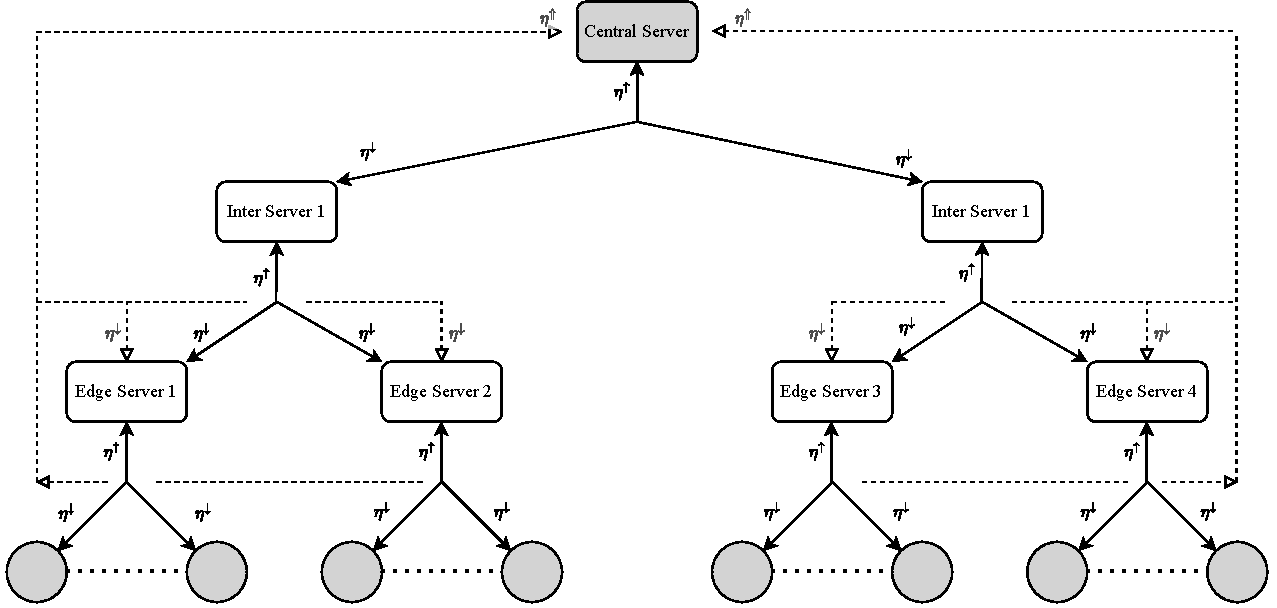
\includegraphics[clip,width=\columnwidth]{plots/Tree_Structure.drawio.pdf}
    \caption[System Diagram]{Example B-HFL system. Solid lines represent communication links, and dashed lines represent conceptual ``residual'' connections. Nodes capable of training, such as clients and the central server with proxy data, are in grey. When model parameters propagate up, nodes merge incoming pseudo-gradients and update their model with learning rate $\eta^\uparrow$. The same happens when parameters flow from parents to child nodes with learning rate $\eta^\downarrow$. Since the dashed lines communicate $0$ to $K$ models, $\eta^\Uparrow$ may represent $0$ to $K$ aggregations using a $\eta^\uparrow$ learning rate.}\label{fig:TreeStructure}
\end{figure}

An example of a B-HFL system, which would be the first deliverable for the second year of my PhD, may be seen in \cref{fig:TreeStructure}. The central server controls a proxy dataset used to train after it performs aggregation. Intermediary servers perform only aggregation. Servers send updates to the parent after every round.

Each node, including the clients, runs at-least two stateful FedOPT server optimisers with separate learning rates, one for the leaf-to-root aggregation and one for parent aggregation. Even if the same leaf-to-root learning rate $\eta^\uparrow$ and root-to-leaf learning rate $\eta^\downarrow$ were to be used for all nodes in the tree or at a given level, the independent server optimiser states would distinguish the aggregation procedure of their node based on historical trends. The central server uses model interpolation with a mixture parameter~\citep{AdaptivePersonalisedFederatedLearning} adapted to its proxy data to merge child updates.

The ``residual'' connections serve different functions between the leaf-to-root and root-to-leaf stages. For the upward stage, they collect the $K=1$ client update with the highest absolute value, thus sending one additional model to the central server per edge server. For the downward stage, they allow the edge servers to directly benefit from the central server's training without relying on averaged intermediate models. While this last component is somewhat superfluous in the small hierarchy shown by \cref{fig:TreeStructure}, it may prove relevant for profound structures. For example, in deep hierarchies, parameters that receive extra training at the central server might get averaged several times before reaching the edge servers and thus influencing the leaves.


\section{Research Directions}\label{sec:proposal:research_directions}
\cref{alg:B-HFL} imposes sufficient structure to create a new family of hierarchical FL systems, opening a series of research directions. These directions can be primarily divided into three types: (a) node aggregation procedures filling in the \textsc{NodeOpt} function, (b) ``residual'' selection procedures filling in the \textsc{SelectResiduals} function, and (c) clustering algorithms which decide how client nodes are divided across the physical or virtual edge-servers. Both node aggregation and ``residual'' selection are expected to be set for types of nodes or levels of the tree, as allowing each node to have a separate aggregation procedure would be difficult to manage. Regarding clustering, relations imposed by the physical communication links and purely conceptual ones must be distinguished as the former are unalterable. Importantly, a physical edge server may contain multiple virtual nodes to which clients may be assigned.

\paragraph{Node Aggregation Procedures} Relevant node aggregation procedures can either be those developed for standard FL or procedures that take advantage of the unique tree structure or available proxy data. FedOPT~\citep{FedOPT} and Iterative Moving Averaging~\citep{UnderstandingModelAveragingInFL} are examples of standard FL algorithms that offer unique \emph{implicit} benefits for this hierarchical structure because they maintain stateful accumulators or previous models, respectively, which permit every server to be distinguished. The smaller number of children of non-edge servers may also enable costly aggregation procedures.  For example, internal nodes having potential proxy data allows them to use model interpolations via either training regularisation~\citep{Ditto} or by using adaptive interpolation rates, as proposed by \citet{AdaptivePersonalisedFederatedLearning}, optimised to the proxy data in order to balance the influence of updates from child nodes, parents nodes, and
from proxy training. Aggregation procedures can also \emph{explicitly} consider the links between nodes. A simple example of this second type is aggregation considering the distance between an ancestor and a ``residual'' descendant. More complex procedures may combine the known hierarchical topology with similarity metrics to create a distance matrix between internal node models and perform graph message passing~\citep{GNNSurvey}, as proposed by \citet{FederatedLearningWithGraph}, to interpolate parameters between all internal nodes.
\paragraph{``Residual'' Selection Procedures} For ``residuals'' to be beneficial during aggregation, they must contain information not already evident in their parent's model. As mentioned, it is well-known that averaging is an imperfect means of aggregating models trained on Non-IID data~\citep{FedAvg,LargeCohorts,OnTheConvergenceOfFedAvgOnNonIIDdata,FedProx} as the directions of different pseudo-gradients may conflict. Additionally, maintaining some degree of diversity in ensembles~\citep{StochasticMultipleChoiceLearningDiverseEnsembles} and parameter averages~\citep{DiverseWeightAveraging} is known to be potentially beneficial. As such, in the case of leaf-to-root ``residuals'', parameters may be selected based on simple metrics like an $l_n$ norm, their per-sample loss, or their relation to each other (e.g., cosine similarity). If necessary for communication efficiency, an average update from the top-K outlier gradients, according to the metric, may substitute selecting multiple ``residuals''.
\paragraph{Clustering Algorithms}  Since the connection between cloud and edge servers or multiple layers of intermediary servers is fixed by physical communication links, the underlying communication hierarchy must also remain fixed, making edge reassignments impossible. However, each physical server can create arbitrarily many internal virtual nodes if it adheres to the structure in \cref{alg:B-HFL}. Thus, each physical server is assumed to have the ability to create internal node hierarchies, and edge servers are assumed to have the ability to create clusters for clients within their geographic area. These properties could be exploited for the creation of a B-HFL dynamic clustering system similar to Auxo~\citep{Auxo} where edge-servers would split into multiple virtual nodes to create clusters for clients to be assigned to; however, unlike Auxo, these clusters would maintain a common parent node and thus share information.
\paragraph{Criteria for Success} Given these research directions, it is essential to consider their impact. The proposed research will be successful in the near term if it leads to published work based on the example system in \cref{sec:proposal:example_system}, at ICLR, MLSys, NeurIPS, or an equivalent conference, as detailed in \cref{sec:timeplan:secondYear}. Within the scope of the whole PhD, B-HFL would be successful if its structure allows for faster convergence to the global optimum by avoiding the diminishing effects of large cohorts, creating a more performant global model, or constructing excellent cluster models through inter-cluster communication. Alternative criteria include achieving similar performance to standard FL algorithms with lower communication costs or obtaining evidence that ``residual'' connections and bidirectional partial aggregation are independently beneficial.
\paragraph{Potential Risks} Considering the previously mentioned criteria, potential risks to the methodology include: (a) the continued proliferation of large models trained on public corpora, which are challenging to federate without extensive GPU resources being available to the clients, (b) a lack of adaptivity in the hierarchical structure. For the first risk, if large models continue to proliferate, efficiently training them in a federated fashion via model splitting would need to be added as a primary research direction. For the second, if the proposed B-HFL structure is too rigid to manipulate and would be thus difficult to apply in a practical FL scenario, it would be preferable to refocus the work entirely on inter-cluster communication through a parent node where the depth of the hierarchy never exceeds that of the example system in \cref{fig:TreeStructure}.



\chapter{Completed Work}\label{sec:completed_work}
The proposal in this document emerged as a natural consequence of research on Personalised Federated Learning and Hierarchical Federated Learning I began during my MPhil in Advanced Computer Science and the first year of my PhD.

\citet{EuroMLSysWorkshop} investigated the trade-off between generalisation and personalisation, which is at the heart of this work, from the perspectives of Fair Federated Learning and its interactions with local adaptation~(fine-tuning) of the federated model post-training. Since Fair Federated Learning attempts to construct a more uniform accuracy distribution for the federated model over the local test sets of clients, the expectation was to either reduce the need for personalization or to provide a better starting point from which to carry it out. The experimental results showed that Fair FL brings no benefits and potential downsides towards later personalization and led to the proposal of a Personalisation-aware FL algorithm that attempts to anticipate the common regularises used during fine-tuning throughout the FL process.

\citet{OperaWorkshop} evaluated the performance of Federated Human Activity Recognition~\citep{HARusingFL_2018} when trained using multimodal data gathered from different sensor types at increasing levels of privacy. It showed that grouping clients based on the type of sensor that produced their training set effectively mitigated the impacts of privacy being required at a human subject, environment, and sensor level simultaneously. It was a direct precursor to Bidirectional Hierarchical Federated Learning as it relied on a two-tiered model structure where each client trained both a group-level model and the global federated model using a mutual learning approach~\citep{DeepMutualLearning}. This work was later extended to consider the adaptability of such two-tiered systems to the addition of a new sensor type~(group) into the federation; the extension was submitted to the \href{https://mobiuk.org/2023}{MobiUK} symposium. Mutual learning was chosen to relate the group-level and global models since it allowed divergent architectures that only shared the output layer. However, despite its success, this training method requires clients to have a high amount of data and local epochs to train both models. The expensive nature of the procedure prompted a move towards a model-averaging approach.

Both of the previous works were implemented in the Flower~\citep{Flower} FL framework; however, the scale of experimentation required for fully validating B-HFL would be unfeasible on the publicly available simulation engine. As such, I have contributed to research on a new engine that doubles Flower simulations' throughput by intelligent ML-based client placement on GPUs. The paper has``High-throughput Simulation of Federated Learning via Resource-Aware Client Placement'' has been submitted to \href{https://sigmobile.org/mobicom/2023/}{Mobicom} and is pending review. All the mentioned works are available as appendices to this proposal.


\chapter{Plan and Timeline}\label{sec:timeplan}

The presented family of Bidirectional Hierarchical Federated Learning algorithms will be developed during the PhD period and will form part of the final PhD thesis. In addition, before the final thesis, it offers opportunities for conference publications that significantly contribute to Federated Learning. Given the novelty of FL in general and hierarchical FL in particular, there is ample room for further developments in the structure of B-HFL as the fields mature.

\section{Second-year Plan}\label{sec:timeplan:secondYear}
The summer period of the end of my first year of the PhD will be dedicated to implementing the example version of B-HFL in the Flower~\citep{Flower} FL framework affiliated with my research group. The framework is currently tuned to standard FL settings and would require heavy API modifications to execute and simulate hierarchical FL effectively. However, the previous work on group-level models for Federated Human Activity Recognition of \citet{OperaWorkshop} and the effective FL simulation engine I contributed to can be the basis for implementing and streamlining the process.

The autumn Michaelmas Term of my second year will have as a main objective the publication of a conference paper based on the example system proposed in \cref{sec:proposal:example_system}. \href{https://iclr.cc/}{ICLR} and \href{https://mlsys.org/}{MLSys} would be appropriate venues. Given the growing importance of LLMs, and the trade-offs recently discovered by \citet{PersonalisationGeneralisationTradeoff} in terms of their generalisation and personalisation abilities with or without pre-trained weights, they represent a natural application for the proposed hierarchical system. Moreover, multilingual text prediction provides a naturally clustered FL application corresponding to real-world scenarios where countries have independent servers for FL and must collaborate at a continental and global level. The study would use a large multilingual BERT model~\citep{RoBERTA} together with two multilingual datasets~\citep[e.g., ][]{XGLUE,mC4} for training. One dataset will be partitioned by language, and the other will be kept as a proxy dataset at the central server, as in \cref{fig:TreeStructure}. The study's goals would be to compare the final accuracy of each model at every level of the hierarchy on the client test sets and the centralised test set created from the proxy dataset. The expectation would be for the model performance on the data of a specific client to be proportional to their proximity to that client in the tree. Alternatively, for the proxy test set and the union of all client test sets, accuracy should be proportional to the proximity to the central server. In addition, ablation studies on the ``residual'' connections, adaptive optimisation, or persistent local models will also be performed together with efficiency comparisons between synchronous and asynchronous node execution at different levels of the tree. Finally, if time allows, the paper could include other naturally-clustered tasks, such as speech recognition for multilingual data.

Following the publication of this work, a natural extension during Lent and Easter terms would be to tackle a setting where clients continuously generate and delete data with limited local storage. The example system would be extended to allow asynchronous training on all nodes, including the leaves, which run parallel to the actual FL component. Each client would generate a data stream while having a fixed internal memory to operate on during training. Real resource constraints and asynchronicity can be modelled using the Raspberry Pi FL cluster at Cambridge ML Systems. This work would be intended for \href{https://sigmobile.org/mobicom/2023/}{MobiCom} or another systems conference. The summer term would include buffer time to account for any new projects spawned from previous ones. This would then be followed up by a further literature review on clustering and model aggregation, an inspection of the code of Auxo~\citep{Auxo}, and the implementation of early prototypes for automatic clustering in B-HFL\@.
\section{Third-year Plan}
During Michaelmas, I would finalise the thesis's literature review and implement an automatic hierarchical clustering system in the vein of Auxo. If successful, this would be intended for a potential publication at ICLR or a later conference.

The beginning of the Lent term will represent the beginning of the thesis write-up considering all work done up to that point. Lent term would then involve exploring different ``residual'' selection criteria and complex aggregation procedures based on the hierarchical structure of the model, assuming that the B-HFL system contains natural or automatically constructed clusters. The findings would be written up for a conference or workshop if successful.

Easter term would be devoted to finishing any work leftover from Michaelmas or Lent. The rest of the time will be devoted to constructing a complete thesis outline and continuing the write-up started during the Lent term. The summer term would be dedicated to finishing the thesis.




% \renewcommand to change default "Bibliography" to "References"
\renewcommand{\bibname}{References}
\cleardoublepage
\phantomsection
\addcontentsline{toc}{chapter}{References}
\bibliographystyle{plainnat}
\bibliography{thesis}



%%%%%%%%%%%%%%%%%%%%%%%%%%%%%%%%%%%%%%%%%%%%%%%%%%%%%%%%%%%%%%%%%%%%%%%%%%%%%%%%
%% Appendix:
%%

\appendix

\chapter{Completed Works}
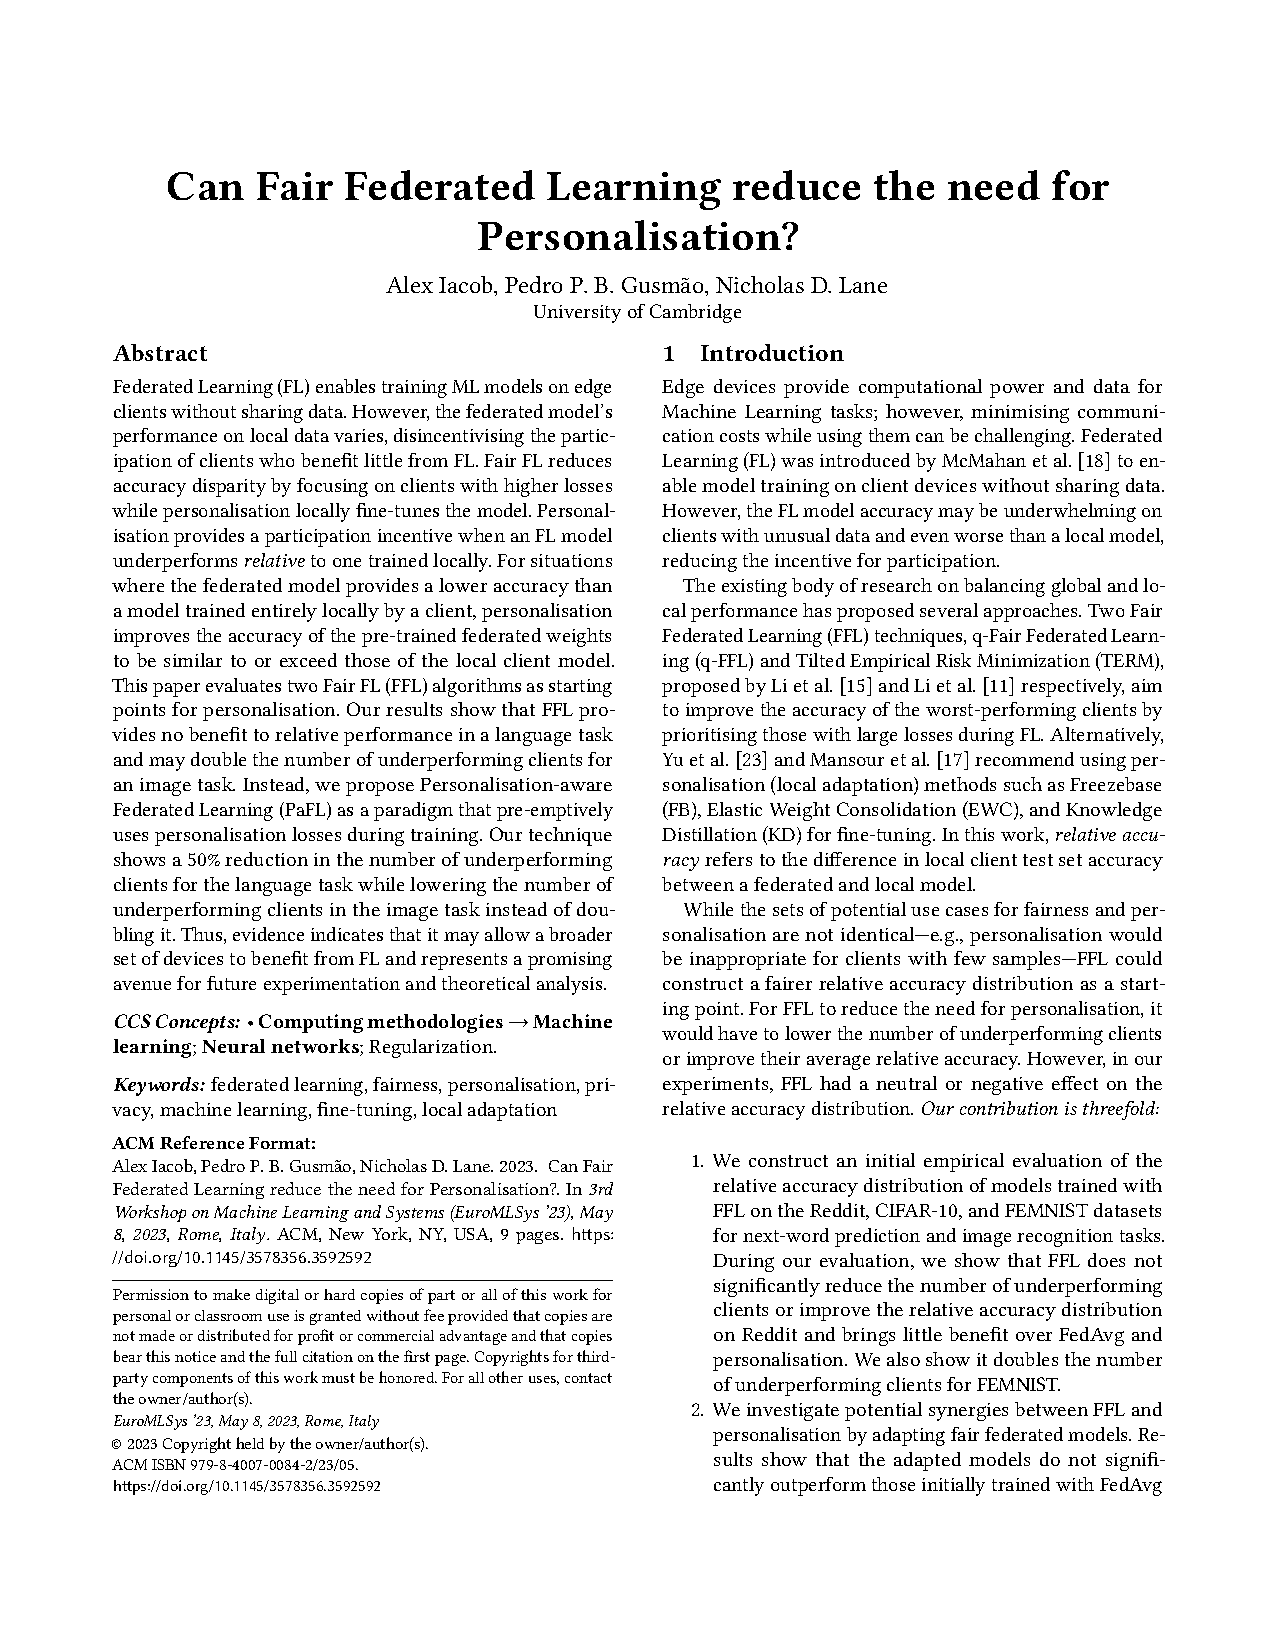
\includepdf[pages=-]{plots/EuroMLSys.pdf}
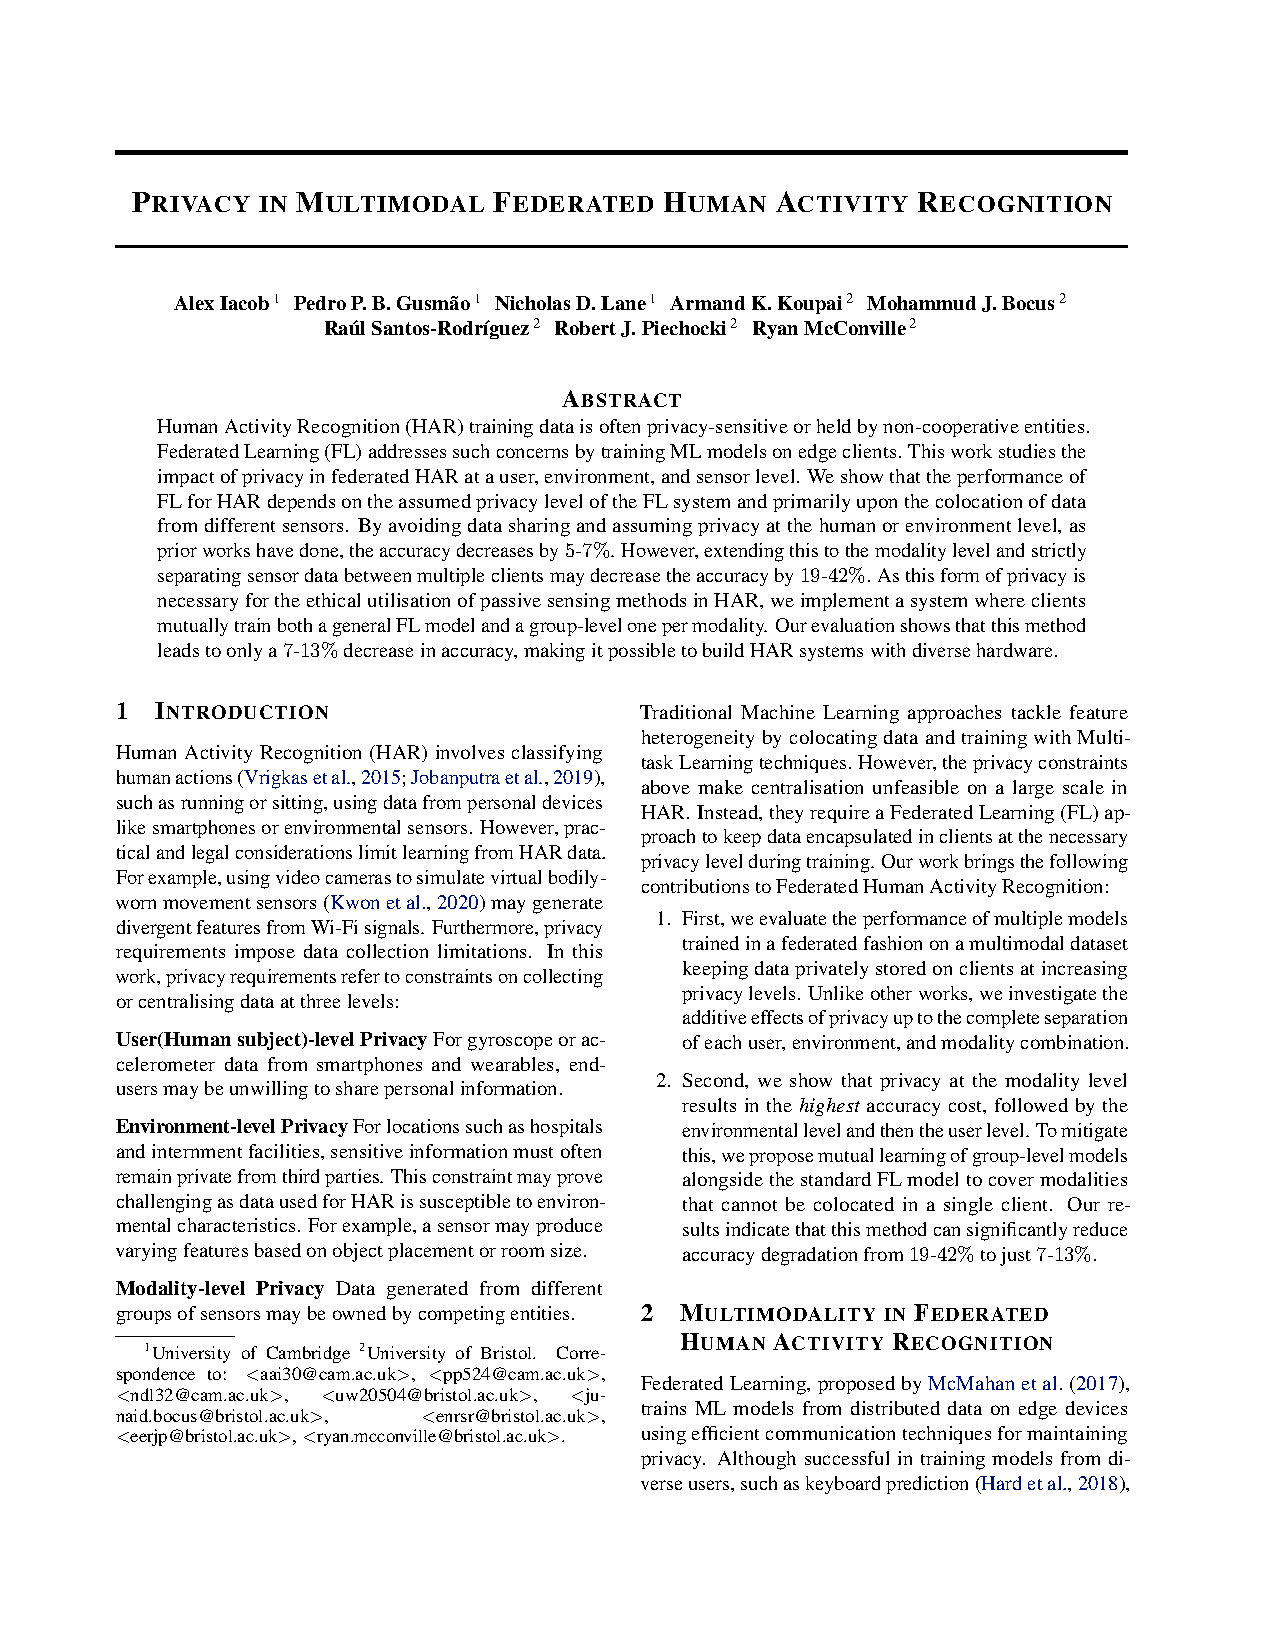
\includepdf[pages=-]{plots/Privacy_HAR_Alex_Iacob_Camera_Ready.pdf}
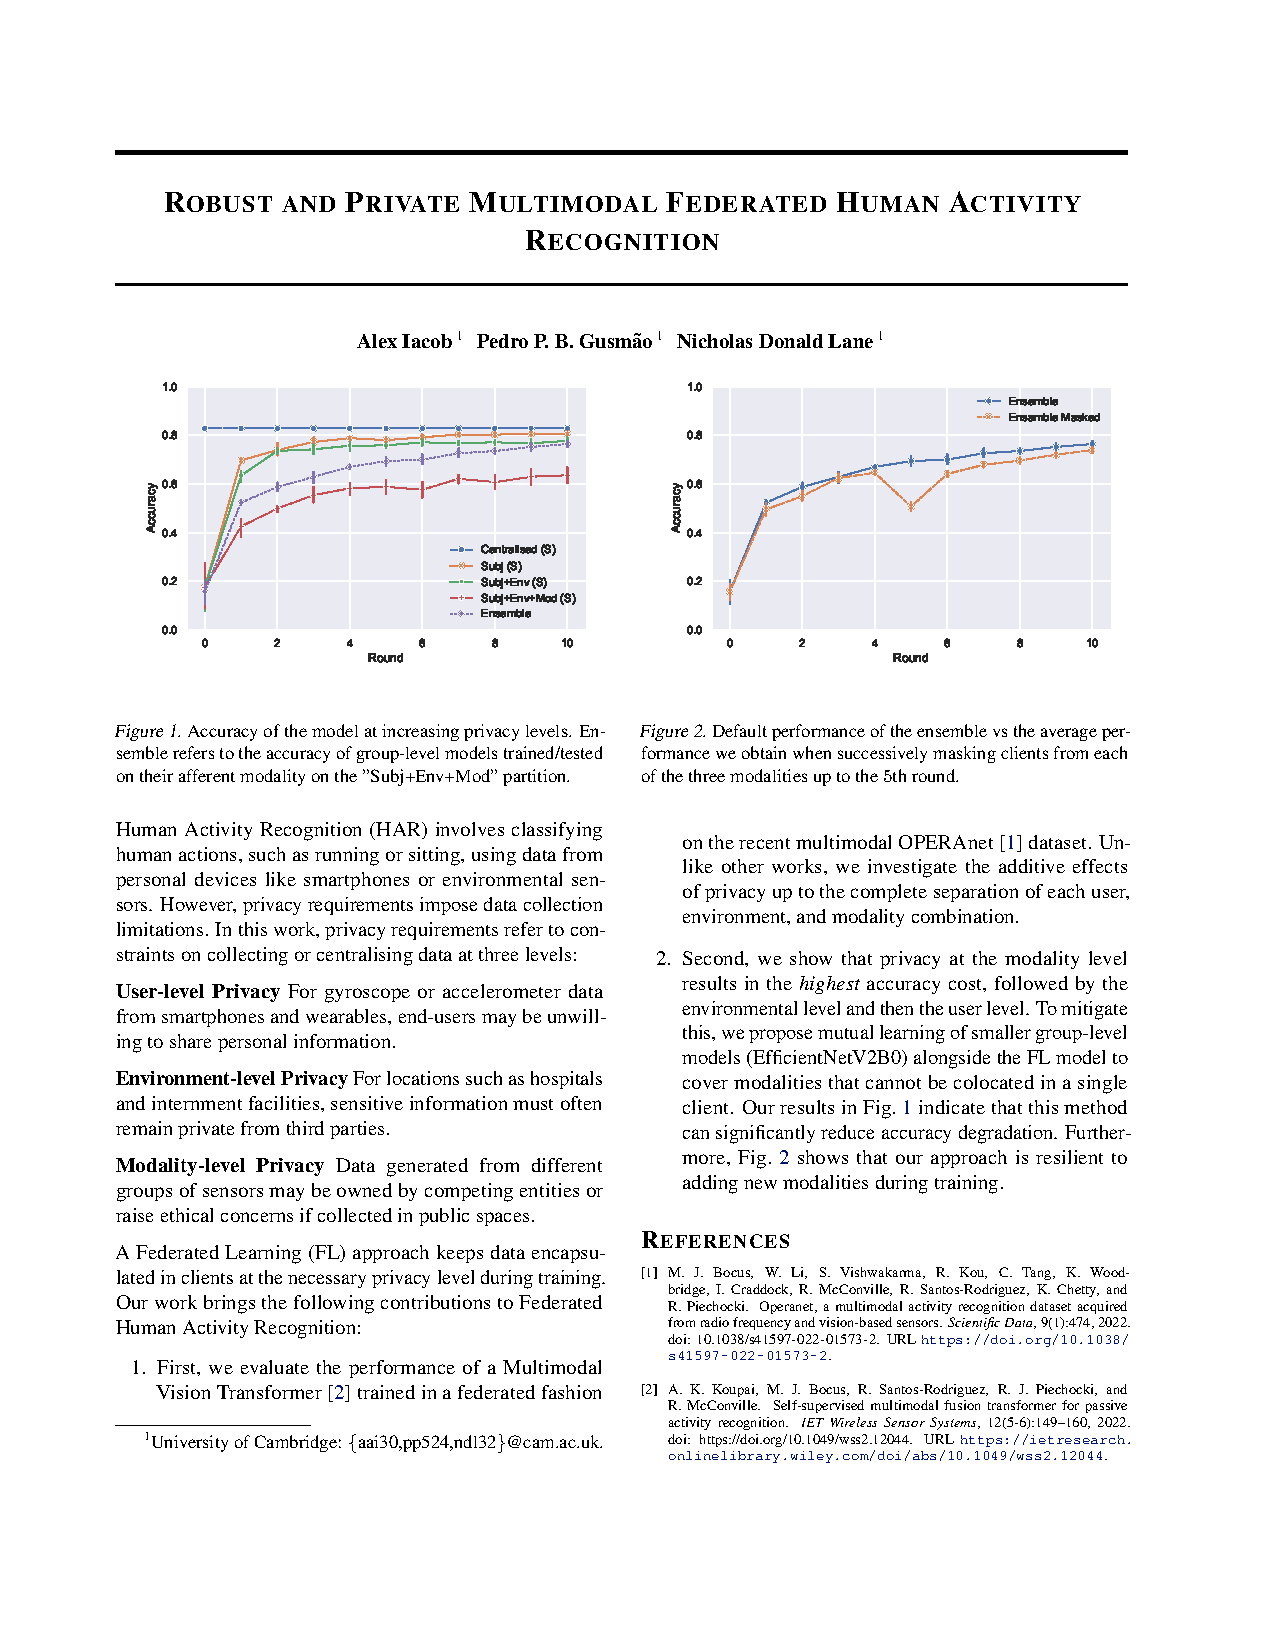
\includepdf[pages=-]{plots/MobiUk.pdf}
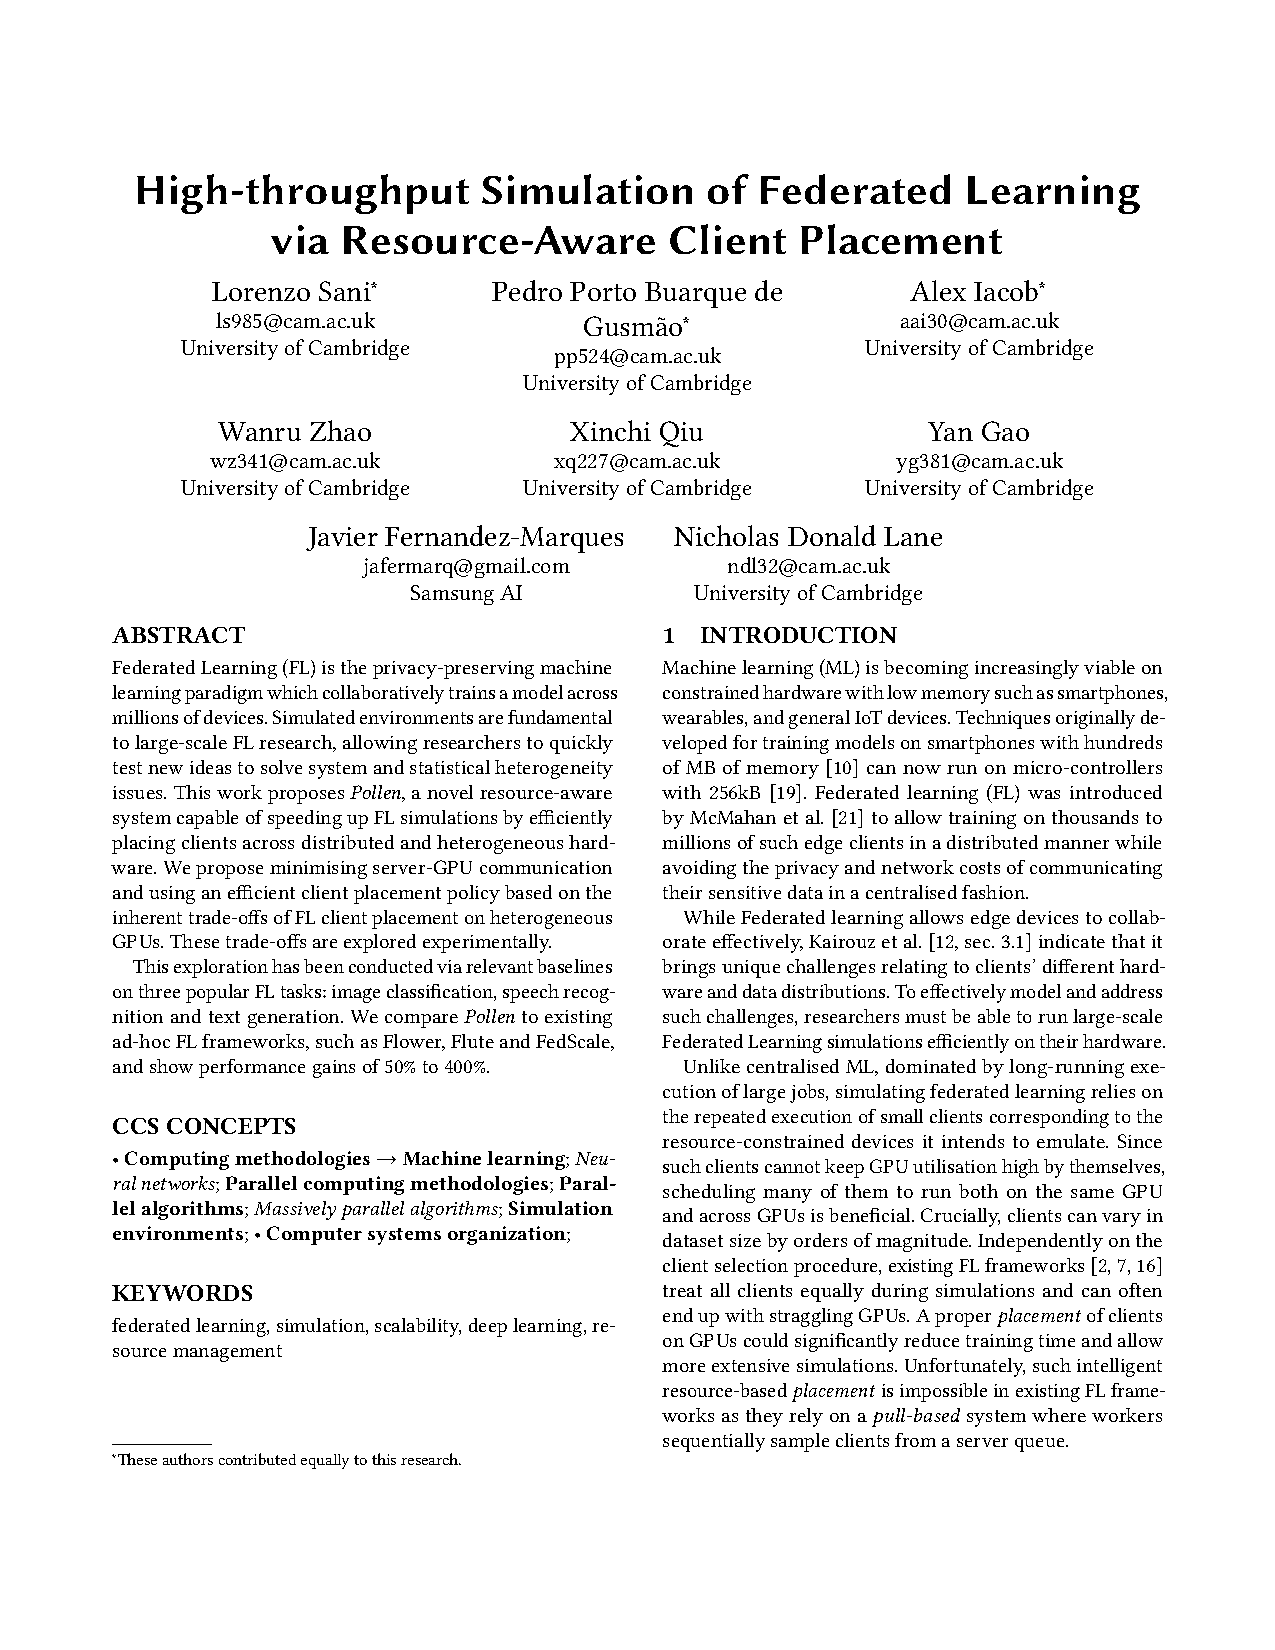
\includepdf[pages=-]{plots/MobiCom_2023 (2).pdf}



%%%%%%%%%%%%%%%%%%%%%%%%%%%%%%%%%%%%%%%%%%%%%%%%%%%%%%%%%%%%%%%%%%%%%%%%%%%%%%%%
%% Index:
%%
\printthesisindex

\end{document}
